% !TEX root = dissertationmain.tex
%Chapter
\chapter{Methodology}
\label{chap:chapter1}

%paragraph with reference in bibligraphy.bib
\paragraph{}Methodology Outline*

%Section
\section{Design}
\label{sec:section1}
\paragraph{}

\paragraph{}give academic justification for choices and include math formulaes
%Section
\section{Implementation}
\label{sec:section2}

%Subsection
\subsection{Subsection} 
\label{ssec:subsection1}


\paragraph{}This is a paragraph located in a subsection.  This paragraph also reference a  Figure~\ref{flow}.

%Figure
\begin{figure}[!t]
\centering
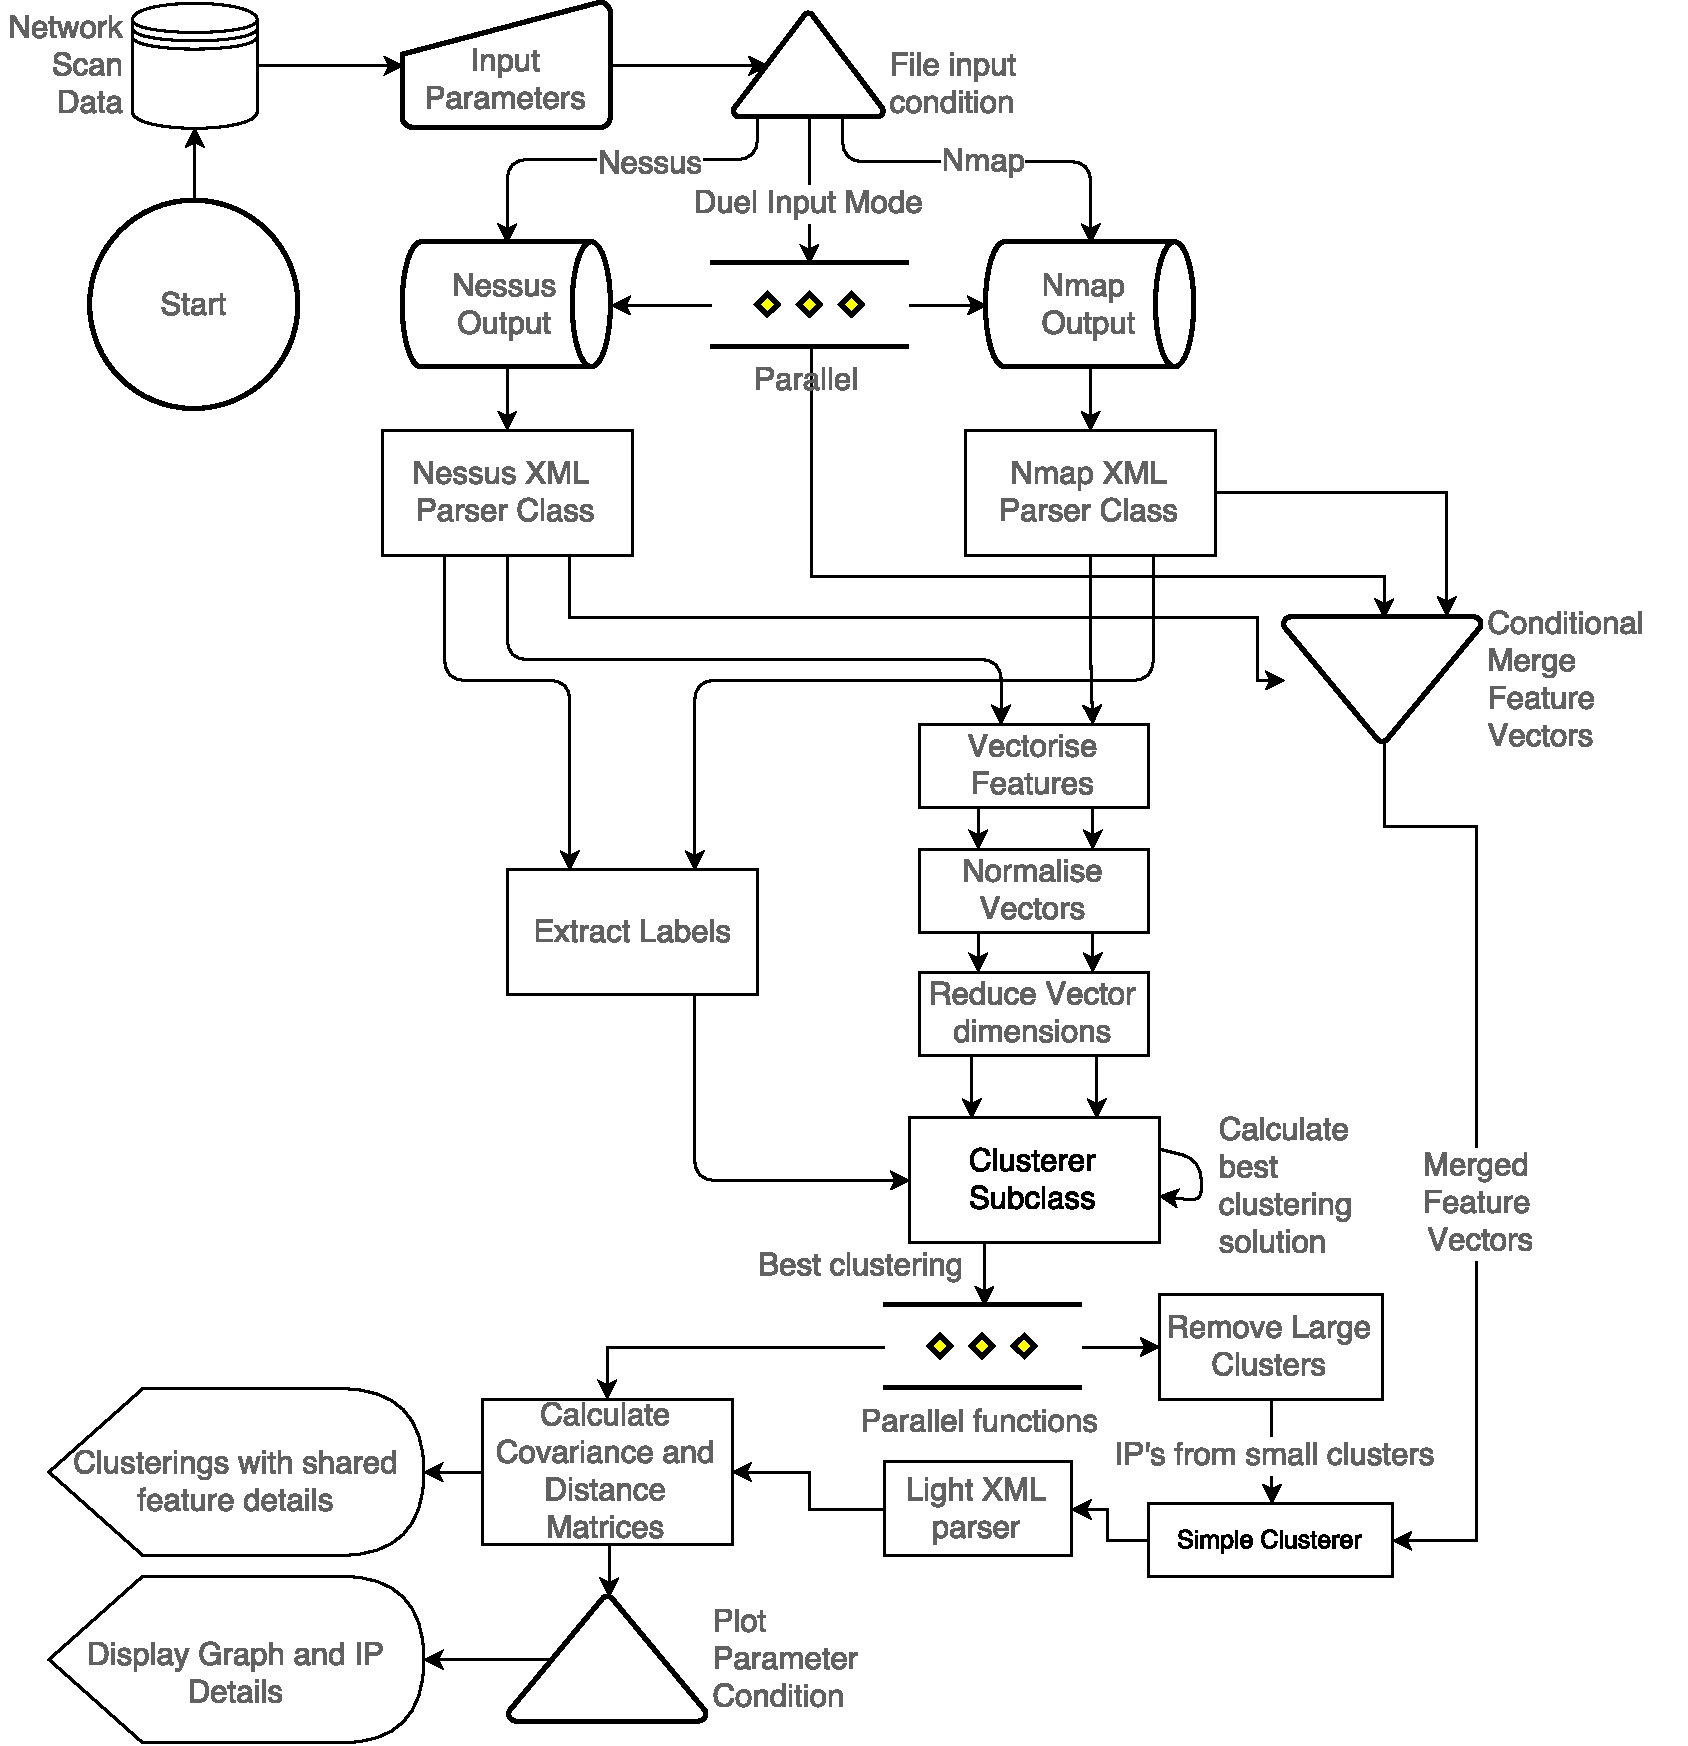
\includegraphics[width=5.5in]{./Figures/flow.pdf}
\caption{Application Infrastructure flow Diagram}
\label{flow}
\end{figure}

%subsection 2
\subsection{Subsection}
\label{ssec:subsection2}

\paragraph{}This paragraph reference another subsection~\ref{sec:section1}.

%Section
\section{Application Brief}
\label{sec:section3}

%Section
\section{Proof of Concept Testing}
\label{sec:section4}


